\section{Mathematical analysis of the structure} \label{c:analysis}
%
In this chapter we present theoretical results of time and space complexity of
the multiset-trie data structure. In the following Section~\ref{s:timecomplexity} 
we discuss the running time complexity of the presented algorithms. First, in 
Section~\ref{ss:mathmodel}, we present our mathematical model that we use 
to describe the distribution of multisets in the multiset-trie and input data. 
Using probabilistic approach and tools from a Galton-Watson process we 
measure the expected cardinality of the multiset-trie in Theorem~\ref{thm:exp_nodes}. 
Further, we derive the expected cardinality of the searched subtree of the 
multiset-trie parametrized by an input multiset in Corollary~\ref{cor:exp_nodes_param}.

In Section~\ref{ss:getall} we discuss the running time complexity of the functions 
\textsc{getAllSubmsets} and \textsc{getAllSupermsets}. We observe that the 
complexity of functions is exponential. Moreover, the worst case running time 
complexity is the same for both functions and its upper bound is the cardinality of 
the multiset-trie.

The remaining "existence" functions are discussed in the Section~\ref{ss:exists}. 
We observe that out of scope of our mathematical model unlike in functions 
\textsc{getAllSubmsets} and \textsc{getAllSupermsets} the mapping $\phi$ has an 
impact on performance of the functions \textsc{submsetExistence} and 
\textsc{supermsetExistence}. In particular, the frequency analysis of the symbols 
from $\Sigma$ in input data determines such a $\phi$ that gives a boost in performance. 

We find that the performance of the functions \textsc{submsetExistence} and 
\textsc{supermsetExistence} in the worst case scenario is also exponential and 
does not depend on the outcome of the functions. We give a quite precise upper 
bound for the worst case running time complexity, which appears to be the same 
for both functions. However, it must be stressed that for the positive outcome an 
exponential behavior holds only on specific cases, such as presence of the emptyset 
in the multiset-trie. 

Finalizing the mathematical analysis, we present the study of space complexity 
of the multiset-trie in the Section~\ref{s:spacecomplexity}. We show that the space 
used for the storage is asymptotically equal to the size of the input data. 

\subsection{Time complexity of the algorithms}\label{s:timecomplexity}
The performance of the functions will be measured by the number of 
visited nodes in a multiset-trie during execution of a particular query by the 
functions \textsc{search}, \textsc{delete}, \textsc{submsetExistence}, 
\textsc{supermsetExistence}, \textsc{getAllSubmsets}, \textsc{getAllSupermsets} 
and the procedure \textsc{insert}.
%

By the design of the multiset-trie, it is easy to see that the functions \textsc{search},
\textsc{delete} and the procedure \textsc{insert} have complexity of $O(\sigma).$
Because $\sigma$ is defined when the structure is initialized and does not depend
on the user input afterwards, the asymptotic complexity of the functions \textsc{search}, 
\textsc{delete} and the procedure \textsc{insert} is $O(1).$ Nonetheless, in the general 
case the complexity is $O(\sigma).$

In what follows, we focus on analysis of the more involved functions:
\textsc{submsetExistence}, \textsc{supermsetExistence}, \textsc{getAllSubmsets}
and \textsc{getAllSupermsets}.

\subsubsection{Mathematical model} \label{ss:mathmodel}
We start with the basics of our mathematical model. Let $\Sigma$ be an alphabet of
cardinality $\sigma,$ such that $\Sigma = \{ 1,2, \ldots, \sigma \}.$ Define $N$
to be the set of all possible multisets that can be inserted in
multiset-trie. Let $n$ be the maximal degree of a node in multiset-trie.
Then the maximal multiplicity of an element in a multiset is equal to $n-1.$
Thus, the number of multisets in a complete multiset-trie is $ |N| = n^{\sigma}.$
%
Let $M$ be a collection of multisets inserted into multiset-trie $\mathcal{M}.$
All the multisets in $M$ are constructed from the alphabet $\Sigma$ according
to the parameters $\sigma$ and $n$. Hence, any multiset $m\in M,$ 
has at most $\sigma$ distinct elements that are members of $\Sigma$ and 
every distinct element in $m$ has multiplicity strictly less than $n.$
%
Because a multiset does not distinguish different orderings, it is assumed, for
simplicity that all elements are ordered in an ascending order. A multiset $m$ is
represented as $\{1^{k_1},2^{k_2},\ldots, \sigma^{k_\sigma}\},$ where $e^{k_e}$
represents an element $e\in\Sigma$ with multiplicity $k_e.$
%

Denote the nodes of multiset-trie on all levels but on $\sigma + 1$ as \emph{internal}
and nodes on leaf level as \emph{leaf} nodes.
%
Observe that every internal non-root node has a degree at least~1. Indeed an
insertion of a multiset requires a construction of a path of length~$\sigma + 1,$
meaning that if an internal node exists in a multiset-trie it must have a degree
at least~1. It also follows that the height of a multiset-trie is always~$\sigma +1$
as soon as at least one multiset is inserted into the data structure.

Our model assumes that all the inserted multisets are chosen with the same probability,
meaning that for some $p\in (0,1)$ the following holds:
\[
P(m\in M) = p, \quad \forall~m\in N.
\]
%
Let $\xi_1, \xi_2, \ldots, \xi_{\sigma+1}$ be random variables such that $\xi_i$
represents the number of nodes in a multiset-trie on $i$-th level. For every node $j$ 
on $i$-th level we assign a random variable $\xi_{ij}$ to be the number of its children, 
such that $j\in[1,\xi_i].$ Then for every $i\in[1,\sigma]$ the following holds:
%
\begin{equation}\label{eq:sum_recursive}
\xi_{i+1} = \sum_{j=1}^{\xi_i} \xi_{ij},
\end{equation}
%
where $\xi_1 = 1.$
%
It is easy to see that the variable $\xi_{i+1}$ can have values in the interval
$[\xi_i,n^{i}]$ and the value of the variable $\xi_{ij}$ is within the interval $[1,n].$
Without conditioning on the existence of any node in multiset-trie, 
it is easy to describe the probability of existence of any individual node.

\begin{lemma}\label{l:prob-node-existence}
Any potential node on a fixed level $i,$ where $i\in \{ 1,2,\ldots, \sigma +1 \}$ exists, %independently of others,
with probability
\begin{equation}
p_i=1-(1-p)^{n^{\sigma + 1 -i}}.
\end{equation}
\end{lemma}
\begin{proof}
Let $v$ be an arbitrary node in a multiset-trie on an arbitrary level $i.$ Consider
the subtree with the root $v$ and call it $v$-subtree. Since the height of the
multiset-trie is $\sigma + 1$ we can calculate the height of the $v$-subtree.
Taking in account that the root node has height 1, the height of the $v$-subtree is
%
\[
h_v = \sigma + 1 - i.
\]
%
A node in a multiset-trie exists if at least one node exists on the leaf level of its
subtree, i.e. a node on the level $\sigma + 1$ that belongs to $v$-subtree. The possible
number of nodes on the leaf level of $v$-subtree can be easily calculated knowing its height.
It is equal to
%
\[
n^{\sigma + 1 - i}.
\]
%
A node at level $\sigma+1$ exists with probability $p,$ where $p = P(m\in M).$
Thus, the probability that there are no nodes on leaf level in $v$-subtree is
%
\[
(1-p)^{n^{\sigma +1 - i}}.
\]
%
The claim follows by taking the complement probability of the above result. 
\hspace*{\fill}\qed
%
\end{proof}

However, in order to determine the distribution of $\xi_{ij}$, one needs a lemma of a different kind.

\begin{lemma}\label{l:prob-children}
Suppose that a node $v$ exists at level $1\leq i\leq\sigma$.
Then the number of its children $\xi_{iv}$ is modeled by a zero-truncated binomially
distributed random variable on parameters $n$ and $p_{i+1}$. In particular,
the probability of node $v$ having $k$ children equals to
\begin{equation}\label{eq:pdf}
P(\xi_{iv} = k) = \frac{\binom{n}{k} (1-p_{i+1})^{n-k}}{1-(1-p_{i+1})^n}
\end{equation}
and the corresponding probability generating function equals to
\begin{equation}\label{eq:generating_func}
G_i(z) = \frac{(1+p_{i+1}(z-1))^n - (1-p_{i+1})^n}{1-(1-p_{i+1})^n}.
\end{equation}
\end{lemma}
\begin{proof}
In order to prove the lemma, we have to show that
$\xi_{iv}\sim\mathcal{B}_0(n, p_{i+1}).$
Consider an arbitrary node $v$ on level $1\leq i\leq\sigma.$ According to the
definition of the multiset-trie a node exists at level $i$ if and only if
it has at least one child. Note that this is not true for the nodes on the leaf
level $\sigma + 1.$ Implies, a node on level $i$ can have
$k\in\{ 1,2,\ldots, n\}$ children. Let $X_0, X_1, \ldots, X_{n-1}$ be random
variables, they are defined as follows:
\[
X_k = \begin{cases}
0 & \textrm{child $k$ of node $v$ does not exist} \\
1 & \textrm{child $k$ of node $v$ exists} \\
\end{cases}
\]
As it was shown in previous Lemma~\ref{l:prob-children}, the distribution of 
$X_k$ is $X_k\sim Bernoulli(p_{i+1}).$ Since our model assumes that all the 
multisets in $M$ are chosen uniformly at random, the variables 
$X_k,X_l$ are independent for $k\neq l.$ But in our case the node $v$ can not 
have 0 children, so the sum $\sum_{k=1}^n X_k$ has a zero-truncated binomial 
distribution:
%
\[
\sum_{k=1}^n X_k \sim\mathcal{B}_0(n,p_{i+1})
\]
%
which completes the proof.
\hspace*{\fill}\qed
\end{proof}
%
Knowing the probability density and probability generating functions of $\xi_{ij}$ 
from Lemma~\ref{l:prob-children}, we now can estimate the number of nodes in 
a randomly generated multiset-trie as follows:
%
\begin{equation}\label{eq:num_nodes}
\mathbb{E}( | \mathcal{M} | ) = \mathbb{E}\left[ \sum_{i=1}^{\sigma+1} \xi_i \right].
\end{equation}
%

%Note that in a real world models multisets in $M$ are not chosen with the same 
%probability. Specifically, in some cases, the probability $P(m\in M)$ varies 
%dramatically and can be even equal to $0.$ For example, if words are mapped 
%to multisets, then the sample space $N$ contains very large multisets. However, 
%most of them will have probability $P(m\in M)=0,$ because a word that would correspond 
%to such a multiset simply does not exist. So, we can safely conclude that multiset-trie 
%is an input sensitive data structure, because the size of multiset-trie $|\mathcal{M}|$ 
%depends on the probability distribution function $P(m\in M).$
%

In order to evaluate~(\cref{eq:num_nodes}) we will use some of the tools from 
a Galton-Watson process, see Gardiner~\cite{gardiner1985stochastic} for 
an introduction.
Using the equations~(\cref{eq:sum_recursive}) and~(\cref{eq:generating_func}) we can 
derive the probability generating function for the random variable $\xi_{i+1}$ as 
\begin{equation}\label{eq:g_rec}
G_{\xi_{i+1}}(z) = G_{\xi_i}(G_i(z)).
\end{equation}
Since there is always precisely one node at the root-level, we have $P(\xi_1 = 1) = 1.$ 
Hence, the probability generating function for the random variable $\xi_1$ is 
\begin{equation}\label{eq:g_xi_one}
G_{\xi_1}(z) = z^1 = z
\end{equation}
which is the initial condition for the recursive equation~(\cref{eq:g_rec}).

\begin{proposition}\label{prop:exp_rec}
The expectation of the random variable $\xi_{i+1}$ can be expressed 
as follows.
\[
\mathbb{E}(\xi_{i+1}) = \mathbb{E}(\xi_i)\mathbb{E}(\mathcal{B}_0(n,p_{i+1}))
\]
for $1\leq i\leq\sigma.$
\end{proposition}
\begin{proof}
Using the following property of probability generating function
\begin{equation}\label{eq:prop_exp-pgf}
G_X'(1^-) = \mathbb{E}(X)
\end{equation}
the expectation for the random variable $\xi_{i+1}$ can be derived in terms of 
the equation~(\cref{eq:g_rec}).
\begin{eqnarray}\label{eq:exp}
\mathbb{E}(\xi_{i+1}) &=& G_{\xi_{i+1}}'(1^-) \nonumber \\
&=& G_{\xi_i}'(G_i(1^-))G_i'(1^-).
\end{eqnarray}
According to~(\cref{eq:pdf}) and~(\cref{eq:generating_func}) the value of $G_i(z)$ at 
$1$ is $1$ and the value of its derivative at $1$ is $\mathbb{E}(\mathcal{B}_0(n,p_{i+1})).$ 
Substituting the values of $G_i(1^-)$ and $G_i'(1^-),$ and applying the 
property~(\cref{eq:prop_exp-pgf}) we complete the proof.
\hspace*{\fill}\qed
\end{proof}
%
From the Proposition~\ref{prop:exp_rec} above and Lemma~\ref{l:prob-children} we 
can conclude that 
\begin{eqnarray}
\mathbb{E}(\xi_{i}) &=& \mathbb{E}(\xi_{i-1})\mathbb{E}\left( \mathcal{B}_0(n,p_{i}) \right) \nonumber \\
& = & \mathbb{E}(\xi_{i-1})\frac{np_{i}}{1-(1-p_{i})^n}.
\end{eqnarray}

\begin{theorem}\label{thm:exp_level}
Let $\mathcal{M}$ be a multiset-trie defined with parameters $n,$ $\sigma,$ and denote the number 
of nodes on every level $i$ by a random variable $\xi_i.$ Furthermore, let all multisets appear in 
$\mathcal{M}$ with equal probability $p\in (0,1).$ Then the expected number 
of nodes on every level of $\mathcal{M},$ i.e. $\mathbb{E}(\xi_i)$ is defined as 
\begin{equation}\label{eq:nodes_level}
\mathbb{E}(\xi_{i}) = n^{i-1} \frac{1-(1-p)^{n^{\sigma +1 -i}}}{1-(1-p)^{n^{\sigma}}}.
\end{equation}
\end{theorem}
\begin{proof}
According to~(\cref{eq:g_xi_one}) the expected number of nodes on the first level is 1. \\
Using $\mathbb{E}(\xi_1) = 1$ and the result from Proposition~\ref{prop:exp_rec}
we get
\begin{eqnarray*}
\mathbb{E}(\xi_{i}) &=& \prod_{j=2}^{i} \frac{n p_j}{1-(1-p_j)^n}
= \prod_{j=2}^{i} n \frac{1-(1-p)^{n^{\sigma +1-j}}}{1-(1-p)^{n^{\sigma + 2 -j}}} \\
&=& n^{i-1} \frac{1-(1-p)^{n^{\sigma +1 -i}}}{1-(1-p)^{n^{\sigma}}}
\end{eqnarray*}
\hspace*{\fill}\qed
\end{proof}

Having derived the expected number of nodes on every level of multiset-trie, the
expected value of the total number of nodes in a multiset-trie can be calculated 
with respect to the parameters $n,$ $\sigma$ and $p.$ This result is obtained in 
the next theorem.

\begin{theorem}\label{thm:exp_nodes}
The expected cardinality of a multiset-trie defined on parameters $n,$ $\sigma$ 
and $p$ can be computed as 
\begin{equation}
\mathbb{E}( | \mathcal{M} | ) = \sum_{i=1}^{\sigma+1} n^{i-1} \frac{1-(1-p)^{n^{\sigma +1 -i}}}{1-(1-p)^{n^{\sigma}}},
\end{equation}
where $r = (1-p)^n,$ so $r\in(0,1).$
\end{theorem}
\begin{proof}
Using the results obtained from Theorem~\ref{thm:exp_level} we compute 
\begin{eqnarray*}
\mathbb{E}( | \mathcal{M} | ) &=& \mathbb{E}\left[ \sum_{i=1}^{\sigma+1} \xi_i \right] \\
&=& \sum_{i=1}^{\sigma + 1} n^{i-1} \frac{1-(1-p)^{n^{\sigma + 1 -i}}}{1-(1-p)^{n^{\sigma}}} \\
\end{eqnarray*}
\hspace*{\fill}\qed
\end{proof}

With the expected number of nodes in a multiset-trie $\mathcal{M}$ obtained from 
Theorem~\ref{thm:exp_nodes}, we can now generalize the result for a subtree 
in $\mathcal{M}$ parametrized by an input multiset $m.$ The subtrees that we 
are interested in are the ones that contain all the submultisets or all the 
supermultisets of $m.$ In order to calculate the expected cardinality of such 
subtrees we need the following definition. 

\begin{definition}\label{def:params}
Let $m = \{ 1^{k_1}, 2^{k_2}, \ldots, \sigma^{k_\sigma} \},$ where 
$e^{k_e}$ is an element $e$ with multiplicity $k_e.$ Let $M_1, M_2$ be 
the subsets of the set $M,$ such that $M_1 = \{ x\in M : x\subseteq m \}$ and 
$M_2 = \{ x\in M : x\supseteq m \}.$
Define $\alpha_i$ and $\beta_i$ as follows 
\begin{equation*}
\alpha_i = \begin{cases}
1, & i=0 \\
\prod_{j=1}^i (k_j+1), & 1\leq i\leq\sigma \\
\end{cases}
\end{equation*} 
and 
\begin{equation*}
\beta_i = \begin{cases}
1, & i=0 \\
\prod_{j=1}^i (n-k_j-1), & 1\leq i\leq\sigma \\
\end{cases}.
\end{equation*}
\end{definition}

The expected cardinality of the subtrees containing the multisets from $M_1$ or $M_2$ 
is defined in the following corollary.

\begin{corollary}\label{cor:exp_nodes_param}
Let $M_1, M_2, \alpha_i$ and $\beta_i$ be defined as in previous Definition~\ref{def:params}, 
then the expected cardinality of a multiset-trie subtree $\mathcal{M}_{M_1}$ that contains all the multisets 
from the set $M_1$ is equal to 
\begin{equation}\label{eq:nodes_sub_param}
\mathbb{E}( |\mathcal{M}_{M_1}| ) = \sum_{i=1}^{\sigma + 1} \alpha_{i-1} \frac{1-(1-p)^{\alpha_{i-1}}}{1-(1-p)^{\alpha_{\sigma}}}.
\end{equation}
The expected cardinality of a multiset-trie subtree $\mathcal{M}_{M_2}$ that contains all the multisets 
from the set $M_2$ is equal to 
\begin{equation}\label{eq:nodes_super_param}
\mathbb{E}( |\mathcal{M}_{M_2}| ) = \sum_{i=1}^{\sigma + 1} \beta_{i-1} \frac{1-(1-p)^{\beta_{i-1}}}{1-(1-p)^{\beta_{\sigma}}}.
\end{equation}
\end{corollary}
%
\begin{proof}
Using the results from Theorem~\ref{thm:exp_level} and Theorem~\ref{thm:exp_nodes} 
we derive the formulas~(\cref{eq:nodes_sub_param}) and~(\cref{eq:nodes_super_param}) 
by specifying the possible number of nodes on every level in the multiset-trie according 
to the multiset $m.$ Note that the formula~(\cref{eq:nodes_level}) assumes that on every 
level but the first one there are $n$ possible nodes. Given submultiset or supermultiset 
query and an input multiset $m$ the number of nodes that will be traversed on level $i$ is 
defined by the number $k_{i-1}+1$ or $n-k_{i-1}-1$ for $i\geq 2.$ On level $i=1$ 
there is only one root node in any multiset-trie $\mathcal{M},$ which always exists 
if $M\neq\emptyset$ and is traversed for any type of query (submultiset and 
supermultiset).
\hspace*{\fill}\qed
\end{proof}

\subsubsection{GetAllSubmsets and GetAllSupermsets}\label{ss:getall}
In this subsection we discuss the running time complexity of the functions 
\textsc{getAllSubmsets} and \textsc{getAllSupermsets}. It is obvious that any 
other algorithm for retrieving all the submultisets or supermultisets has worst 
case running time complexity at least $O(|M|).$ Hence, the functions 
\textsc{getAllSubmsets} and \textsc{getAllSupermsets} have the worst case 
running time complexity $O(|\mathcal{M}|).$ Indeed, the case when the algorithms 
retrieve all the multisets stored in a multiset-trie by traversing the whole structure 
can be easily constructed. 

Consider the function \textsc{getAllSubmsets}. The function takes some multiset 
$m$ as an input argument. Then it returns a set of multisets $\{x\in M : x\subseteq m \}$ 
from the multiset-trie $\mathcal{M}$. Having a multiset $m$ set to the largest 
possible multiset in $N$ (it can also be larger) 
\[
m = \{ 1^{n-1},2^{n-1},\ldots, \sigma^{n-1} \}
\]
the whole multiset-trie is traversed during the \textsc{getAllSubmsets} query.

Now let us consider the function \textsc{getAllSupermsets}. Similarly, the function 
takes a multiset $m$ as an input argument. However, in this case it returns the 
set of multisets $\{ x\in M : x\supseteq m \}$ from the multiset-trie 
$\mathcal{M}.$ In order to obtain a traversing of all the multiset-trie one must set 
$m$ to the smallest possible multiset, i.e. an empty multiset
\begin{equation*}
m = \{ \emptyset \} = \{ 1^0,2^0, \ldots, \sigma^0 \}.
\end{equation*}

Thus, we can conclude that the worst case running time complexity of the 
functions \textsc{getAllSubmsets} and \textsc{getAllSupermsets} is $O(\mathbb{E}( |\mathcal{M}| )).$ 
According to the Theorem~\ref{thm:exp_nodes} the expected number of visited 
nodes in the worst case is 
\begin{equation*}
O(\sum_{i=1}^{\sigma+1} n^{i-1} \frac{1-(1-p)^{n^{\sigma +1 -i}}}{1-(1-p)^{n^{\sigma}}}).
\end{equation*}
According to the Theorem~\ref{cor:exp_nodes_param} the worst case running 
time complexity given an input multiset $m$ for the function \textsc{getAllSubmsets} is 
\begin{equation*}
O(\sum_{i=1}^{\sigma + 1} \alpha_{i-1} \frac{1-(1-p)^{\alpha_{i-1}}}{1-(1-p)^{\alpha_{\sigma}}})
\end{equation*}
and for the function \textsc{getAllSupermsets} is 
\begin{equation*}
O(\sum_{i=1}^{\sigma + 1} \beta_{i-1} \frac{1-(1-p)^{\beta_{i-1}}}{1-(1-p)^{\beta_{\sigma}}}).
\end{equation*}

%Taking into account that $\sigma |M| \geq |\mathcal{M}|,$ we can say that the 
%running time complexity is $O(\sigma |M|).$ However, this is a very rough upper 
%bound, which overestimates the complexity a lot. 

\subsubsection{SubmsetExistence and SupermsetExistence}\label{ss:exists}
We start the analysis of the functions \textsc{submsetExistence} and 
\textsc{supermsetExistence} with an observation. Our theoretical model assumes 
that all the multisets are inserted into multiset-trie at random. It was already concluded 
that the probability distribution function $P(m\in M)$ has an impact on the size of 
mulitset-trie $\mathcal{M}.$ Moreover, this distribution influences on the performance 
of the functions \textsc{submsetExistence} and \textsc{supermsetExistence} even more. 

For a real world model, such that $P(m\in M)\neq const$ the performance of the search 
algorithms directly depends on the number of nodes on every level $\xi_i.$ When 
the search functions check if a multiset is in multiset-trie the complete path that 
corresponds to that multiset is checked. Knowing that fact the search can be optimized 
during the construction of a multiset-trie. 

Recall that a multiset-trie is defined on parameters $n,$ $\Sigma,$ $\sigma = |\Sigma|$ 
and $\phi.$ Let the frequency of an element $e$ in a multiset $m$ be the multiplicity of 
$e$ in $m,$ denoted by $\emph{mult}_m(e).$ Then the frequency of an element $e$ 
can be defined as a sum $\sum_{m\in M} \emph{mult}_m(e).$ According to the frequencies 
of elements in $\Sigma,$ the performance of the multiset-trie can be optimized by 
the mapping $\phi : \Sigma \rightarrow I.$ Indeed the ordering of elements by their 
frequencies has an influence on the performance.
%
The frequency of an element $e\in\Sigma$ affects the distribution of $\xi_{\phi(e)}$ 
as follows. The larger the frequency of $e$ the larger the number of nodes on 
$\phi(e)$ level. 
So, if the number of nodes on lower levels is greater than on higher levels, then 
the search functions will discard complete paths that do not satisfy the query 
faster. Hence, the closest match will be found faster.

%
%\begin{lemma}\label{l:frequency}
%Let $M$ be a collection of multisets. Let the frequency of an element $e$ in a 
%multiset $m$ be the multiplicity of $e$ in $m,$ denoted by $\emph{mult}_m(e).$ 
%Then the frequency of an element $e$ is the sum 
%\[
%\sum_{m\in M} \emph{mult}_m(e).
%\] 
%According to the frequencies of elements in $\Sigma,$ the performance of the 
%multiset-trie can be optimized. In particular, the mapping $\phi : \Sigma \rightarrow I$ 
%must order elements by their frequencies as follows. The smaller the frequency of 
%an element the smaller its index.
%\end{lemma}
%%
%\begin{proof}
%The frequency of an element $e\in\Sigma$ affects the distribution of $\xi_{\phi(e)}$ 
%as follows. The larger the frequency of $e$ the larger the number of nodes on 
%$\phi(e)$ level. 
%So, if the number of nodes on lower levels is greater than on higher levels, then 
%the search functions will discard complete paths that do not satisfy the query 
%faster. Hence, the closest match will be found faster.
%\end{proof}
%%

Let us now switch back to our mathematical model and note that the influence 
of the mapping function $\phi$ in our model has inessential impact on performance, 
because all the multisets are equally likely and the whole domain $N$ is used for 
sampling multisets. 

Consider both functions \textsc{submsetExistence} and \textsc{supermsetExistence}. 
Whenever the result is \emph{false}, i.e. no multiset in $M$ is 
a submultiset or supermultiset of an input multiset $m,$ both functions in the 
worst case visit all the nodes in $\mathcal{M}$ but the nodes on leaf level. 
Of course such a case would be very rare assuming a random input model, but 
it can be constructed as follows. 

Consider the function \textsc{submsetExistence}. Then given an input multiset 
$m = \{ 1^{k_1}, 2^{k_2}, \ldots, \sigma^{k_\sigma} \},$ the collection of inserted 
multisets $M$ must be equal to $M = \{ x\in M : k_{x,\sigma} > k_{m,\sigma} \}.$ 
Analogically for the function \textsc{supermsetExistence} with an input multiset 
$m = \{ 1^{k_1}, 2^{k_2}, \ldots, \sigma^{k_\sigma} \},$ the collection of inserted 
multisets $M$ must be equal to $M = \{ x\in M : k_{x,\sigma} < k_{m,\sigma} \}.$ 

Thus, the worst case running time complexity of the functions 
\textsc{submsetExistence} and \textsc{supermsetExistence} is $O(|\mathcal{M}| - |M|).$ 
According to Theorem~\ref{thm:exp_nodes}, this value is 
\begin{equation*}
O(\sum_{i=1}^{\sigma} n^{i-1} \frac{1-(1-p)^{n^{\sigma +1 -i}}}{1-(1-p)^{n^{\sigma}}}).
\end{equation*}
According to Theorem~\ref{cor:exp_nodes_param} the worst case running 
time given an input multiset $m$ for the function \textsc{submsetExistence} is 
\begin{equation*}
O(\sum_{i=1}^{\sigma} \alpha_{i-1} \frac{1-(1-p)^{\alpha_{i-1}}}{1-(1-p)^{\alpha_{\sigma}}})
\end{equation*}
and for the function \textsc{supermsetExistence} is 
\begin{equation*}
O(\sum_{i=1}^{\sigma} \beta_{i-1} \frac{1-(1-p)^{\beta_{i-1}}}{1-(1-p)^{\beta_{\sigma}}}).
\end{equation*}
Note that the summation goes only up to $\sigma$ and not up to $\sigma + 1$ as 
in the Theorem~\ref{thm:exp_nodes} or in the Theorem~\ref{cor:exp_nodes_param}.

As for the case when the outcome of the functions \textsc{submsetExistence} and 
\textsc{supermsetExistence} is \emph{true} one has to guarantee the termination 
of the algorithm at some node on the leaf level. The worst case scenario can be 
constructed in the same way as for the \emph{false} outcome but with two more 
multisets in $M.$ The first multiset is the empty multiset. With the empty multiset 
the function \textsc{submsetExistence} will visit the same amount of nodes as for 
the \emph{false} case plus one more for the empty multiset. The second multiset 
is the maximal possible multiset from $N.$ In this case the function \textsc{supermsetExistence} 
will also visit the same amount of nodes as for the \emph{false} case plus one more 
for the maximal multiset. Hence, the worst case running time complexity for both 
outcomes (\emph{true} and \emph{false}) is the same.

\subsection{Space complexity}\label{s:spacecomplexity}
As in any efficient algorithm there is always some trade-off between space and 
time complexity. While offering efficient sub- and supermultiset queries an 
additional space must be provided for multisets storage. Clearly, the cardinality 
of the set $M$ is smaller than the size of $\mathcal{M},$ because the number 
of multisets in $\mathcal{M}$ is equal to the number of nodes only on the leaf 
level. The figure~\ref{f:exp-nodes} demonstrates the relation between the number 
of multisets stored and the number of nodes needed for storage, where parameters 
$\sigma$ and $n$ are $26$ and $10,$ respectively.

\begin{figure}[h!]
\center
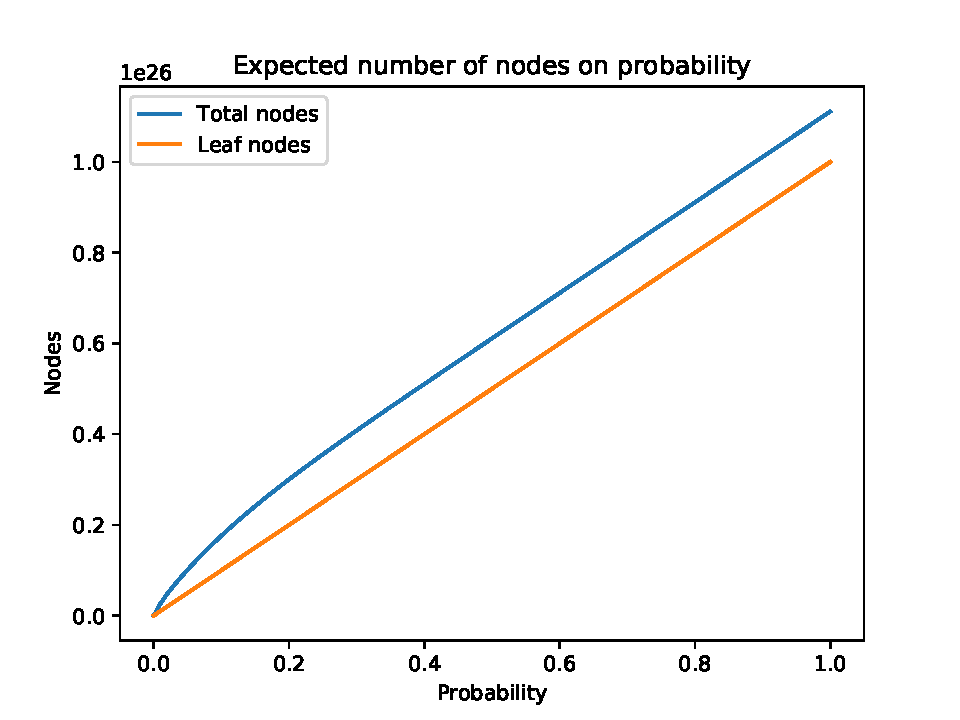
\includegraphics[width=.4\textwidth, keepaspectratio]{exp-nodes-on-probab.pdf}
\caption{$\mathbb{E}(|\mathcal{M}|)$ and $\mathbb{E}(|M|)$ on probability.}
\label{f:exp-nodes}
\end{figure}

As we see on the figure~\ref{f:exp-nodes} the value of $|\mathcal{M}|$ is slightly 
shifted with respect to the value of $|M|.$

Now we demonstrate a more descriptive comparison between $|\mathcal{M}|$ and 
$|M|.$ Figure~\ref{f:ratio-exp-msets} shows the ratio between the expected cardinality 
of a multiset-trie $|\mathcal{M}|$ and the actual number of multisets stored $|M|$ for 
parameters $n$ and $\sigma$ being $10$ and $26$ respectively.

\begin{figure}[h!]
\center
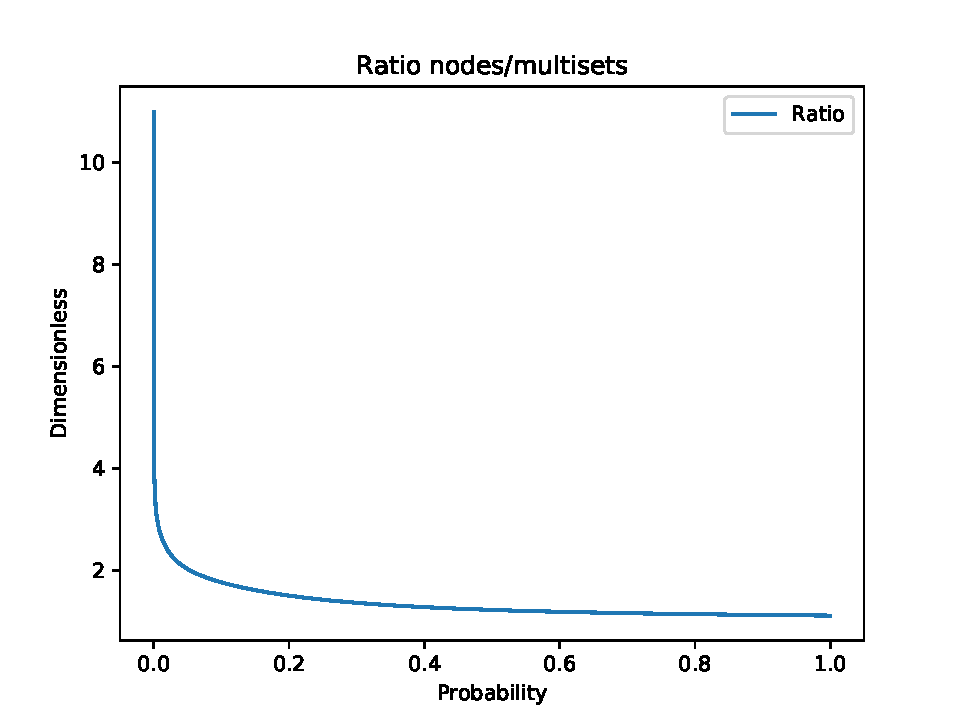
\includegraphics[width=.4\textwidth, keepaspectratio]{ratio-exp-nodes-and-msets-on-prob.pdf}
\caption{Ratio $\mathbb{E}(\frac{|\mathcal{M}|}{|M|})$ on $p.$}
\label{f:ratio-exp-msets}
\end{figure}

Note that analyzing the graph on figure~\ref{f:ratio-exp-msets} we can safely 
say that the upper bound for the ratio is $\sigma + 1.$ The argument holds, 
because of the limit 
\begin{equation}
\lim_{p\rightarrow 0^+} \mathbb{E}(\xi_i) = 1,
\end{equation}
where $\xi_i$ is the number of nodes on $i$-th level and $1\leq i \leq \sigma + 1.$ 

However, the ratio $\sigma + 1$ can be obtained only with a very small cardinality 
of the set $M,$ in particular $|M| = 1.$ In order to obtain such a case the 
probability $p$ must be at most $\frac{1}{n^\sigma}.$

The lower bound for the ratio is obviously at $p=1$ and is equal to 1
\begin{equation}
\lim_{n,\sigma \rightarrow\infty} \frac{n^{\sigma + 1} - 1}{n^\sigma (n-1)} = 1.
\end{equation}

Since the ratio $\sigma + 1$ can be obtained for a very specific case only and 
with a small increase of probability the ratio drops rapidly it can be concluded 
that the space complexity of the multiset-trie is $O(|M|).$





